\section*{Import}

\subsection*{Import report}

\begin{itemize}
  \item[] \textbf{Trigger:} User interaction with CMS window
  \item[] \textbf{Precondition:} Assert that user has logged in
  \item[] \textbf{Path:}
    \begin{enumerate}
      \item User clicks Import Report on navigation bar
      \item User selects the debt report file to be imported
      \item User clicks ``Create Import'' button
      \item User is redirected to list of imports page, where the import is shown as processed
    \end{enumerate}
  \item[] \textbf{Requirements:}
    \begin{enumerate}
      \item The debt report file should be processed
      \item All debts included in the file should be created in the database
      \item The debts that are in the database and not in the file should be marked as paid
    \end{enumerate}
  \item[] \textbf{Screenshots:} \\
    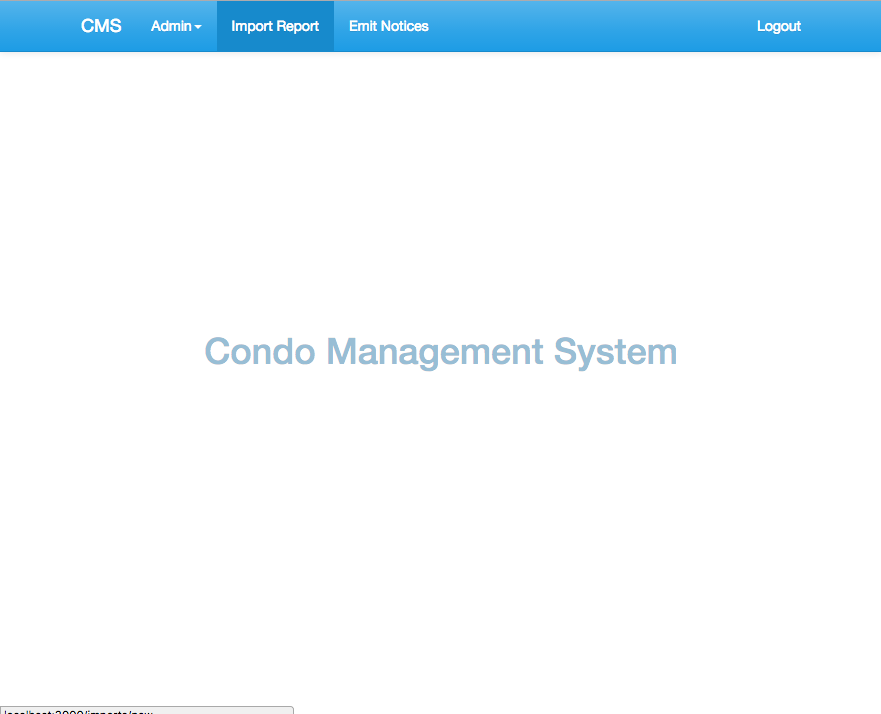
\includegraphics[scale=0.25]{./images/ss/import/1.png}
    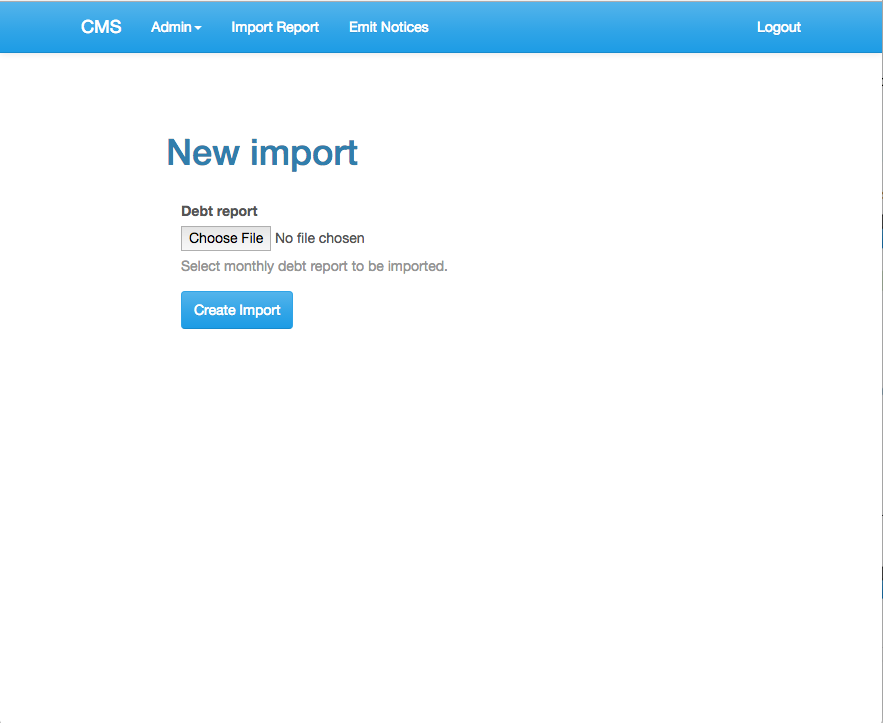
\includegraphics[scale=0.25]{./images/ss/import/2.png}\\
    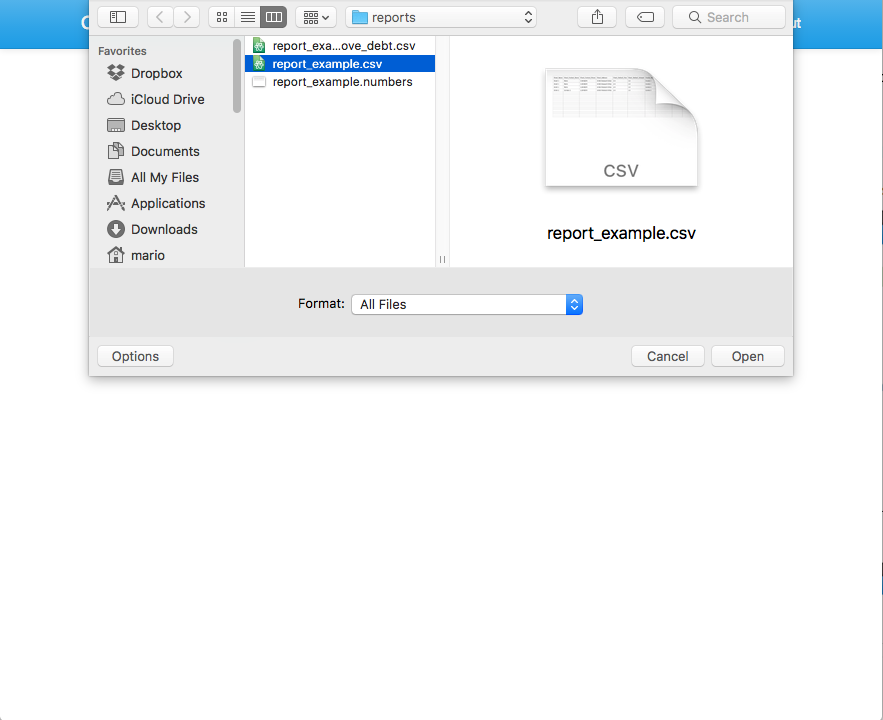
\includegraphics[scale=0.25]{./images/ss/import/3.png}
    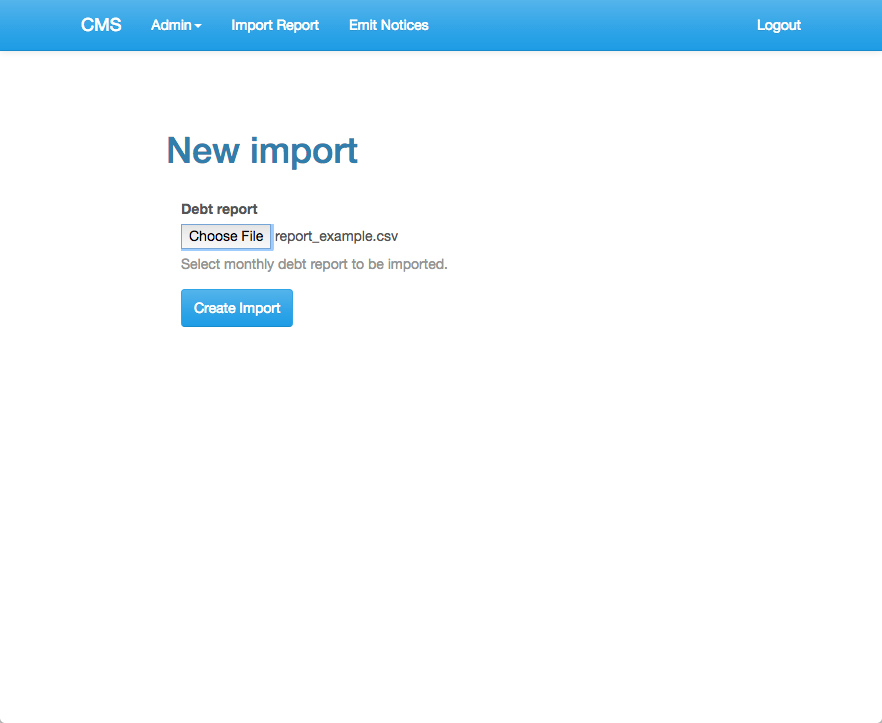
\includegraphics[scale=0.25]{./images/ss/import/4.png}\\
    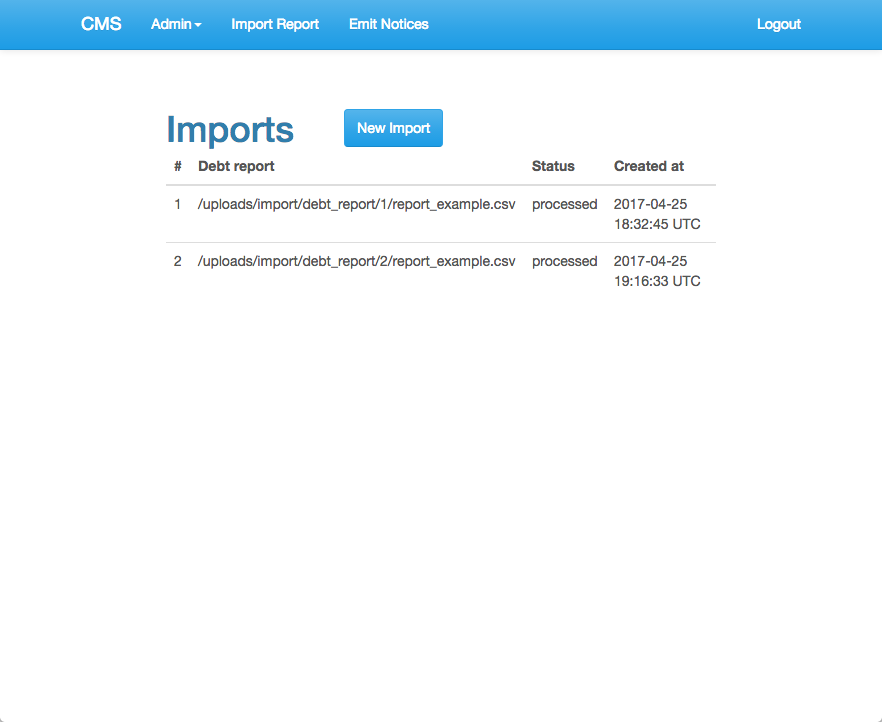
\includegraphics[scale=0.25]{./images/ss/import/5.png}
\end{itemize}
